\documentclass[12pt]{amsart}

\addtolength{\hoffset}{-2.25cm}
\addtolength{\textwidth}{4.5cm}
\addtolength{\voffset}{-2.5cm}
\addtolength{\textheight}{5cm}
\setlength{\parskip}{0pt}
\setlength{\parindent}{15pt}
\usepackage[ngerman]{datetime}

\usepackage{amsthm}
\usepackage{amsmath}
\usepackage{amssymb}
\usepackage[colorlinks = true, linkcolor = black, citecolor = black, final]{hyperref}

\usepackage{graphicx}
\usepackage{multicol}
\usepackage{ marvosym }
\usepackage{wasysym}
\usepackage{tikz}
\usetikzlibrary{patterns}

\newcommand{\ds}{\displaystyle}
\DeclareMathOperator{\sech}{sech}


\setlength{\parindent}{0in}

\pagestyle{empty}

\begin{document}

\thispagestyle{empty}

{\scshape \today} \hfill {\scshape \large Ziel-Definition} \hfill {\scshape Bachelor These}
 
\smallskip

\hrule

\bigskip

\section*{{\bf Titel/Aufgabenstellung}}
\begin{itemize}
\item[(15.Juni)] Die Automatisierung des Knowledge Managements der fachlichen Software-Architektur in einem X-Team mit agiler Organisationsstruktur
\item[(22.Juni)]Untersuchung der Kopplung in einer Aws-Ressourcen Microservice-Landschaft mit Hilfe einer Graph-Datenbank
\item Untersuchung der Kopplung in einer Aws-Ressourcen Microservice-Landschaft 
\bigskip
\item[(30.Juni)] Untersuchung der Kopplung in einer Aws-Ressourcen Microservice-Landschaft mit agiler Organisationsstruktur
\item[(11.Juli)] Ist schwerfällige Kommunikation in einer agilen Organisationsstruktur ein Symptom für zu hoher Kopplung in einer Microservice Landschaft.
\textbf{\item[(12.Juli)] Schwerfällige Kommunikation als Symptom für zu hohe Kopplung in einer Microservice Landschaft.}
\end{itemize}

\bigskip



\bigskip
\section*{{\bf Einleitung - Problem}}
Das Projekt Deep-See in einem Unternemhem soll die Monlitische und schwerfällige Software Landschaft durch eine modulare leichter wartbare Microservice Landschaft ablösen. Doch sind Architekturentscheidungen auch hier maßgeblich verantwortlich für die Wartbarkeit und ... .
Eine Herausforderung in einem MS System ist die Kopplung der Systeme untereinander, also x-team weite Abhängigekeiten zwischen den Domainen so klein wie möglich zu halten. Hier für wird eine eine klare Trennung der Context grenzen vorrausgesetzt. Werden die Fachlichen komponeten aber unzureichend geschnitten entsteht ein zu hoher Grad der Abhängigkeit macht die Kommunikation zäh und langwierig. Teams untereinader merken nach der zeit einen höheren Kommunikationsaufwand aber auf enterprise Ebene kommt die schwerfälligkeit erst an wenn das Projekt auf rot steht. 

Doch stellt sich die Frage in wie weit die Symptome abzubilden sind auf die Kopplung der Domains. 

Die Kommunikation der Teams wird in dem MS-Teams Gruppen festgehalten. Die Vernetzung der Teams kann so repräsentativ abgebildet werden .. und analytisch im lauf der der Projekt Entwicklung betrachte werden. 
Um die Kommunikation auf die service landschaft abzubilden muss auch in der Komponenten archtiktur eine historie abgebildet werden. also hardware updates müssen festgehalten und Deepsea weit zusammen getragen werden.


\bigskip

Im Zeitraum meiner Bachelor Arbeit möchte ich die Updates der Komponenten Wöchtenlich zusammen tragen und diese dann mit dem Kommunikations-Aufwand in kritischen Kopplungs-Bereichen vergleichen. 
Die Gruppen Kommunikation ist eine Metrik im Projekt die nicht zu vernachlässigen. 
Das Setup soll helfen Entscheidungen zu treffen, und unstimmigekeiten in der Architektur zu refactorn.

\section*{{\bf Fragen}}

\medskip

\begin{enumerate}

\item Was ist das Problem?
\item Ab wann ist zu häufige Kommunikation, Anzeichen für zu hohe Kopplung?


\end{enumerate}




\medskip

\newpage

\begin{center}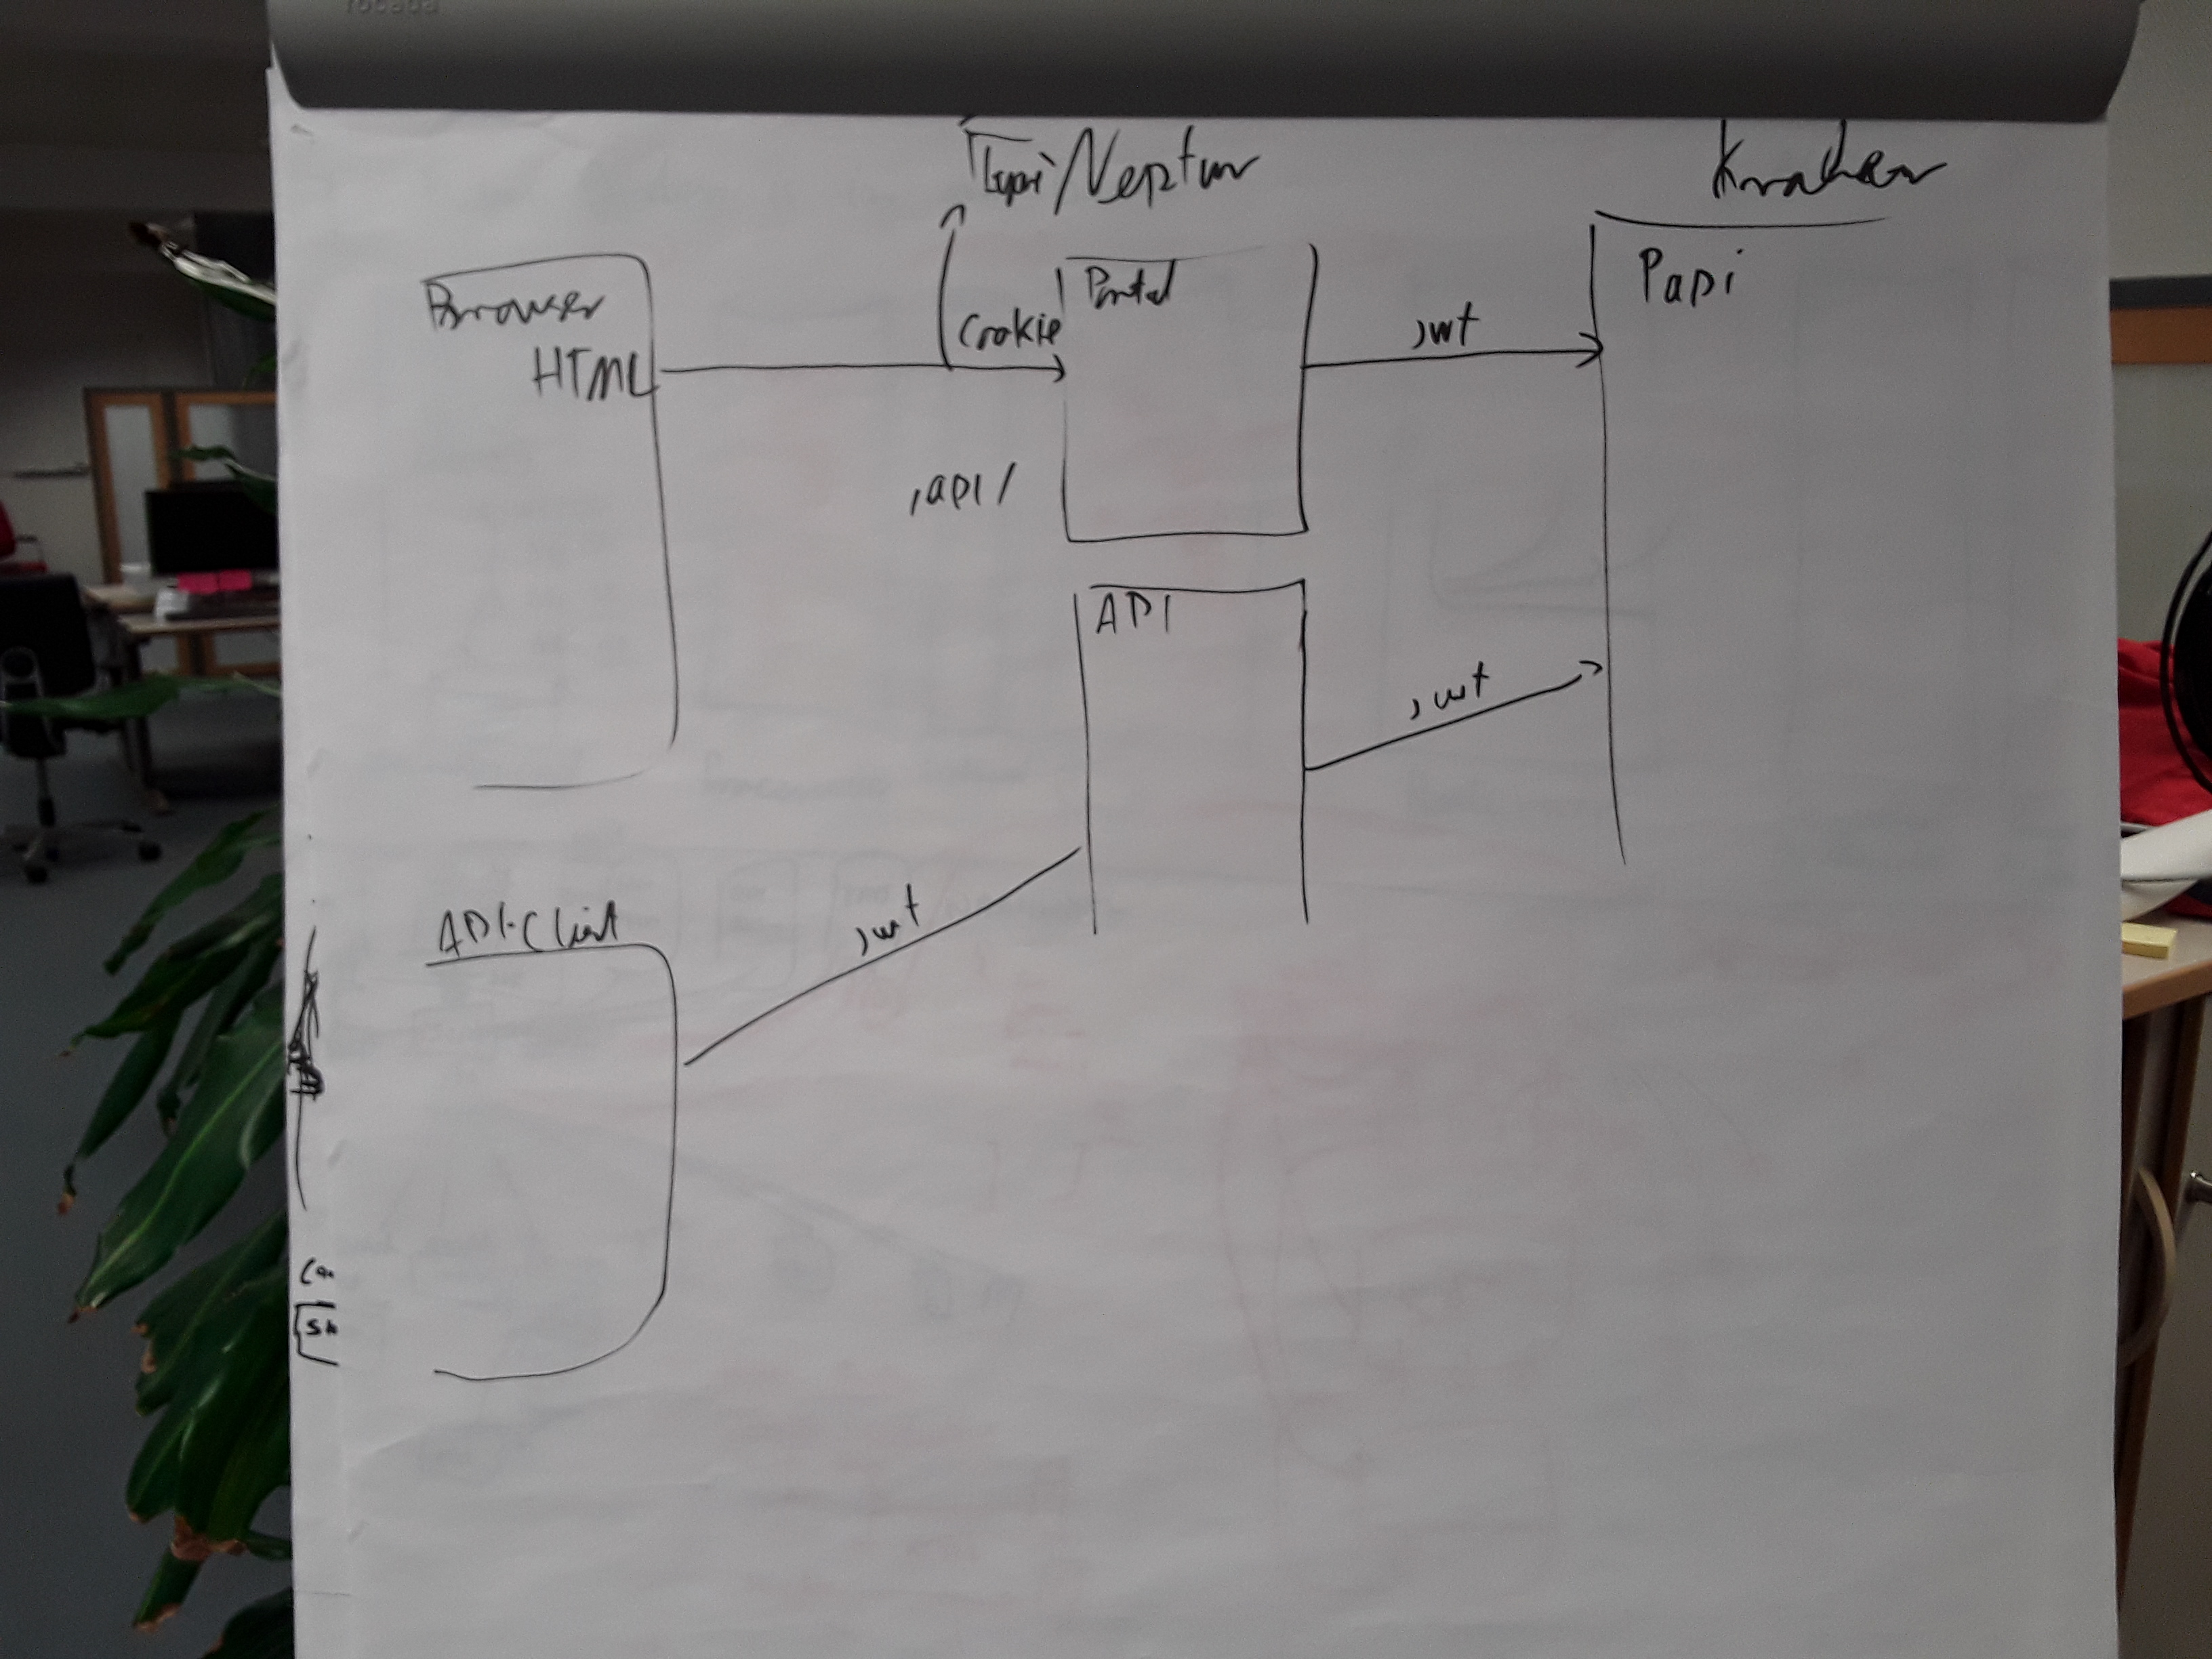
\includegraphics[scale = 0.14]{whith-board _1.jpg}\end{center}

\end{document}